\documentclass[11pt]{article}
\usepackage{acl2013}
\usepackage{url}
\usepackage{latexsym}

\usepackage{fontspec}
\usepackage{xunicode}
\usepackage{xltxtra}

\setmainfont[Mapping=tex-text]{Times New Roman}

%\setlength\titlebox{6.5cm}    % You can expand the title box if you
% really have to

\title{Optimising Morphological Analyser Automata Using Morphological Structure
and Automatically Induced Flag Diacritics}

\iffalse
\author{Senka Drobac \\
Department of Modern Languages \\
PO Box 24 \\
00014 University of Helsinki \\
  {\tt senka.drobac@helsinki.fi} \\\And
  Tommi A Pirinen \\
Departmet of Speech Sciences\\
PO Box 9\\
00014 University of Helsinki\\
  {\tt tommi.pirinen@helsinki.fi} \\}
\fi

\date{\today}

\begin{document}
\maketitle
\begin{abstract}
    Flag diacritics are a historical method of optimising finite-state networks
    by combining identical structures with differing parts. Traditionally the
    feature has required linguists to write the optimisation of the graph by
    hand alongside morphological descriptions. In this paper we present a novel
    method of discovering ideal flag positions automatically based on the
    morpheme strucuture implicit in the language description. With this
    approach we have gained 200~\% decrease in size of finite-state networks
    with no speed penalties on the application phase.
\end{abstract}

\section{Introduction}

The finite-state automata are optimal way of encoding morphological analysers
of natural languages. The automata made for large-scale language materials can
often grow to be too large for some use cases. These automata can be optimised
by recognising equivalent sub-graphs in the automaton, and combining them using
special symbols called flag diacritics to determine the correct entrance and
exit paths. Typical way of applying flag diacritics now requires a linguist to
provide the compiler with the positions for these flags. However, there are two
major problems with this kind of approach: firstly linguists are not very good
in knowing the structure of finite-state networks that will become from
lexicographical-morphological descriptions, secondly the addition of flag
diacritics to these descriptions makes them unreadable and unmanageable since
the amount of non-linguistic data in the linguistic description increases. This
article seeks to address the problem using an algorithm for inducing the ideal
flag positions from the linguistic morpheme structure of the analyser that is
implicitly present in the description. 

One of the reasons why flag diacritics have been so cumbersome in the past,
is their two-fold nature. On the other hand they are there to optimise the
finite-state automaton structure, e.g. in~\cite{karttunen2006numbers}, on the
other hand they are the primary method of describing non-contiguous 
morphological constraints~\cite{beesley1998constraining}. If they are applied
on the constriction of separated morphotactic dependencies, the effect on
optimisation is at best haphazard, and the resulting description does not
look very linguistically motivated or maintainable as computational description.

The paper is organised as follows: In the section~\ref{sec:background} we
introduce the flag diacritics and optimisation problems of finite-state 
automata. In the section~\ref{sec:methods} we show the algorithm for automatic
flag induction we use and describe flag elimination and size measurements we
use. In section~\ref{sec:data} we briefly go through the existing language
descriptions we use to show the differences between hand-written flag
diacritics by expert dictionary writers and our algorithm. In 
section~\ref{sec:evaluation} we show the effects of applying our algorithm
to the size and efficiency of the finite-state automata. In~\ref{sec:discussion}
we evaluate the pros and cons of our approach and lay out future improvements,
and finally in section~\ref{sec:conclusion} we tie the article together by
verifying what we set out to study.

\section{Background}
\label{sec:background}

Finite state morphology~\cite{beesley2003finite} is the state-of-the-art in
writing morphological analysers for natural languages of the whole range of
typologically varying morphological features. The practical finite-state
approach in this frame is build around two practical concepts: writing
lexicographical descriptions of the language using a syntax called lexc, and
writing morphophonological variations in regular expression rules. In this
paper we study the use of lexicographical structure as framed by lexc. Lexc
itself is a simple right-linear phrase structure grammar formalism. In
linguistic terms this means approxiamtely the following: we have concept of
lexicon, which refers to set of morphemes. Each of these morphemes defines a
continuation, which determines a set of morphemes that can come after it. And
these are the only two things there are. 

If think of Finnish morphology for example, nominal inflection is built neatly
from left to right with morphemes. In figure~\ref{fig:lexc-fin} there is a 
lexc representation of Finnish words \emph{talo} `house' and \emph{asu}
`clothing' and \emph{kärry}, and nominal suffixes \emph{n} (singular genitive),
\emph{lle} (singular allative) and \emph{ksi} (singular translative). The
structure of the grammar starts from the \texttt{Root}, each of the nouns in
root set of morphemes continues rightwards to \texttt{NOUNCASES} set of 
morphemes, and each case morpheme continues towards the special \texttt{\#}
lexicon signifying the end of a word-form.

\begin{figure}
    \centering
    \begin{verbatim}
    LEXICON Root
    talo NOUNCASES ;
    asu NOUNCASES ;
    kärry NOUNCASES ;

    LEXICON NOUNCASES
    n # ;
    lle # ;
    ksi # ;
    \end{verbatim}
    \caption{Simplified part of Finnish lexc grammar description
    \label{fig:lexc-fin}}
\end{figure}

Finnish was used as an example in Karttunen's paper on flag diacritics in
optimisation~\shortcite{karttunen2006numbers}. In this paper, he showed that
the optimisation quality of wisely selected flag diacritics is significant;
from 20,498 state automaton to 1,946 state one. The article describes Finnish
numerals, which have the feature of requiring agreeing inflection in free
compounding, and this can be achieved by allowing all compounds and restricting
the combinations by flags instead of lexicon structure. Article does not
unfortunately show examples or re-producable description of the lexicographical
data, but to our experience there are no available morphologies that show
similar compression quality, so it can be considered towards the upper bounds
of what such compression can achieve.
 

\section{Methods}
\label{sec:methods}

Flag diacritics are special multi-character symbols which are interpreted during runtime. They have special syntax: \verb+@operator.feature.value@+, where operator is one of the available operators (P, U, R, D, N, C), feature is name of a feature provisionally set by user and value can be any value held in feature, also provisionally defined ~\cite{beesley2003finite}.

In this paper, we will use only two types of flag diacritics: positive setting (\verb+@P.feature value@+) and require test (\verb+@R.feature value@+). While positive setting flag only sets the feature to its value, require test flag invokes testing if the feature is set to the designated value.
For example, \verb+@P.LEXNAME.Root@+ will set feature \verb+LEXNAME+ to value \verb+Root+. If later in the path occurs request test flag \verb+@R.LEXNAME.Root@+, the invoked test will succeed and that path will be considered as valid. 

Our algorithm is based on the finding that adjacent morph combinatorics can
be expressed with finite-state flags like this:

Eliminating flags is done by

Measuring automata sizes with

\begin{figure*}
    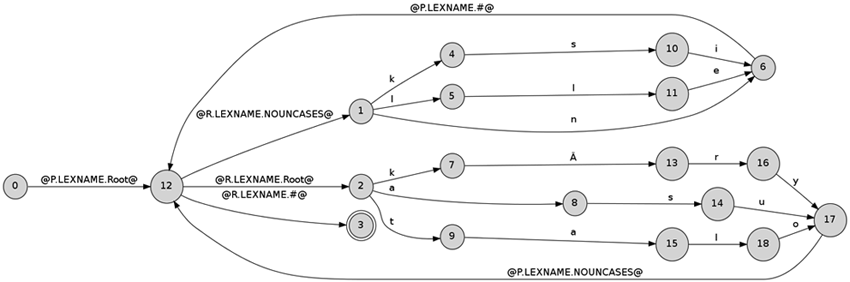
\includegraphics[width=\textwidth]{transducer.png}
     \caption{Simplified part of Finnish lexc grammar description with automatic flags
     \label{fig:lexc-fin-flag}}
\end{figure*}

\section{Data}
\label{sec:data}

We measure the success of our algorithm using real-world, large scale language
descriptions. For this purpose we have acquired freely available, open source
language descriptions from University of Tromsa's language 
repository~\cite{moshagen2013building}. The languages selected are:

\section{Evaluation}
\label{sec:evaluation}

To evaluate the algorithm, we measure the propoportional size gains that are
achieved by the flags we introduce as compared to the equivalent automaton
without the induced flags, and we contrast these results to the ones that have
been attained by having linguists manually determine the flag positions and
their logic. Since introduction of flags always causes an overhead in the
application time of the automata, we also measure the average running speed
of the automata with our flags to get the trade-off ratios.

In table~\ref{table:sizes} there are sizes.

\begin{table}
    \centering
    \begin{tabular}{|l|r|r|r|}
        \hline
        \bf Language & \bf With flags & \bf Original & \bf \% \\
        \hline
        \bf Greenlandic & 8400635 & 261074412 & 3,4\%  \\
        \bf North Saami & 6789658 & 9152930 & 74\%  \\
        \bf Erzya & 2801339 & 3333669 & 84\%  \\
        \bf Komi Zyryen & 2315384 & 2719971 & 85\%  \\
        \bf South Saami & 3147213 & 3600902 & 87\%  \\
        \bf Lule Saami & 3639278 & 4381573 & 87\%  \\
        \bf German & 32678 & 25836 & 126\%  \\
        \hline
    \end{tabular}
    \caption{Sizes of transducers with and with-out automatic flags (in bytes); Percentage shows size of the flagged transducer in comparison to the original
    \label{table:sizes}}
\end{table}


In table~\ref{table:speed} there are speeds.

\begin{table}
    \centering
    \begin{tabular}{|l|r|r|r|}
        \hline
        \bf Language & \bf Original & \bf With flags & \bf Words \\
        \hline
        \bf Greenlandic & 13 s & 164 s  & 764823  \\
        \bf Lule Saami & 1 s & 5 s  & 21262  \\
        \hline
    \end{tabular}
    \caption{Sizes of automata with and with-out flags (in words per second)
    \label{table:speed}}
\end{table}

In table~\ref{table:tradeoff} we have summarised the actual tradeoffs.

\begin{table}
    \centering
    \begin{tabular}{|l|r|r|r|}
        \hline
        \bf Language & \bf Original & \bf Elim. flags & \bf Ours \\
        \hline
        \bf English & 100 & 1,000 & 1  \\
        \hline
    \end{tabular}
    \caption{Trade-off proportions size-to-speed
    \label{table:tradeoff}}
\end{table}


\section{Discussion}
\label{sec:discussion}

The results of this study show/indicate that .......
Surprisingly, no differences were found in ......
There are several possible explanations for this result.

\subsection{Future Directions}
\label{subsec:future-directions}

This is an optimistic thing so we thought that automatic induction of flags
shoulda work nicely for other neat things too. Hyperminimisation based on
morphophonology would be cool. Also, graph-structure. And other things.

\section{Conclusion}
\label{sec:conclusion}

In this article we showed that by using morphologically motivated flags we can
improve the size of the automata by factor of 1000. This way we can prevent
linguist from doing optimisation work in vain and as an added bonus the
linguistic descriptions stay closer to linguistics, and remain more readable.

\iffalse
\section*{Acknowledgments}

We thank our colleagues and we got funding.
\fi

\bibliographystyle{acl}
\bibliography{fsmnlp2013flags}




\end{document}
